%% START NEW SECTION
\section{Causal Bayesian Network}
\subsection{Background and Definition}
\begin{frame}{Assumptions}
\begin{itemize}[<+->]
\item Causal Markov Condition
	\begin{itemize}
	\item Every variable is independent of its non-descendants given its parents
	\item Factorization: $P(X_1,\ldots,X_n)=\prod_iP(X_i\,|\,Parents(X_i))$
	\end{itemize}
\item Faithfulness: causal structure fully determines independences
\item Acyclic: needs to be defined in problem setting
\item Causal sufficiency
	\begin{itemize}
	\item Assume no latent common cause
	\item For efficient learning, also for causal interpretation of output
	\end{itemize}
\end{itemize}
\end{frame}
\begin{frame}{Causal Bayesian Network}
\begin{definition}
Given a set of variables ${X_1,\ldots, X_n}$, a Bayesian network is
a probabilistic graphical model $B = (\mathcal{G}, \Theta)$, where $\mathcal{G}=(V,E)$ is a
directed acyclic graph (DAG) and $\Theta$ is the set of the
parameters in all conditional probability distributions (CPDs).
\end{definition}
A Bayesian network $B$ is said to be causal when do intervention on any subset $X\subseteq V$, i.e., do(X), 
resulting in a set of interventional distributions $P_x$, denoted by $P_*$, and the following three conditions hold:
\begin{itemize}
\item $P_x$ is Markov relative to $\mathcal{G}$
\item $P_x(v_i)=1$ for all variables $v_i\in X$
\item $P_x(v_i\,|\,pa_i)=P(v_i|pa_i)$ for all variables $v_i\notin X$
\end{itemize} 
\end{frame}
\begin{frame}{An example}
\begin{figure}
\centering
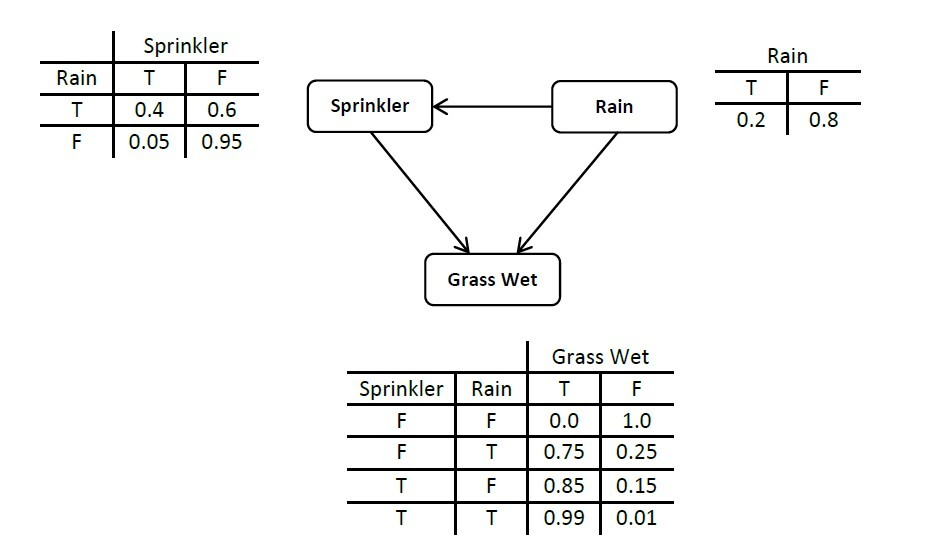
\includegraphics[scale=0.4]{imgs/bnexample}
\end{figure}
\end{frame}
\subsection{Learning Bayesian Network}
\begin{frame}{Problem Setting}
\begin{block}{Goal}
Given a dataset $\mathcal{D}$, try to learn the graph $\mathcal{G}$ and the
parameters of all conditional probability distribution $\Theta$.
\end{block}\pause
\begin{itemize}
\item[] \textbf{Traditional method}
	\item First step: structure learning
	\item Second step: parameter estimation conform to the inferred structure 
\end{itemize}
\end{frame}
\begin{frame}{Structure learning}
\begin{columns}
\begin{column}[t]{5cm}
\textbf{Constraint based}\\
Run conditional independence tests in 
data and find a DAG faithful to 
them. 
\begin{itemize}
\item \textit{Methods:} SGS, PC, TPDA, CPC 
\end{itemize}
\textbf{Hybrid}\\
Combining both constraint based and score based.
\begin{itemize}
\item \textit{Methods:} MMHC, CB, ECOS
\end{itemize}
\end{column}
\begin{column}[t]{5cm}
\textbf{Score based}\\
Find a DAG by maximizing the
posteriori probability given the data.
\begin{itemize}
\item \textit{Methods:} K2, Sparse Candidate, GBPS, BIC/AIC
\end{itemize}
\end{column}
\end{columns}
\end{frame}
\begin{frame}{Parameter Estimation}
Given the structure $\mathcal{G}$ learned from last step, factorization
will be applied according to local terms governed by parameters $\theta_i$
\begin{center}
$P(X_1,\ldots,X_n)=\prod_iP(X_i\,|\,Pa_i, \theta_i)$
\end{center}
Any parameter estimator will work here, e.g, MLE, MAP
\end{frame}
\begin{frame}{Some problems in BN Learning}
\begin{itemize}
\item Search space is exponentially large in high dimension
\item Too many conditional tests
\item Local minimum
\item Parametric form needed
\item Missing values
\item Latent variables
\item Hybrid node type
\end{itemize}
\end{frame}